% タイトル
\chapter{CPUについて}
\vspace{-45pt} %高さ調整
\begin{flushright}
  {\bf \large 理工学部 電気電子工学科 3回生} \\ \vspace{3pt} %所属
  {\bf \large 本田 卓} \\ \vspace{30pt} %名前
\end{flushright}

% 序論
\section*{はじめに}
今の私たちの生活にスマホ、パソコンなどの電子機器は欠かすことのできないものになっている。そして、その電子機器一つ一つの中には必ずCPUが内蔵されている。CPUは電子機器にとっては頭脳のような役割を果たすもので、電子機器を動作させるために最も重要なものといっても過言ではない。大学生になると一人一台パソコンを持っていると思うので、そのパソコンにどのCPUが使われているかを気にして購入した人ならいくつかのCPUの性能や価格の違いなどに詳しい人もいるかもしれない。しかし、そのような場合、それぞれのCPUを比べてどれが良い、どれが悪いかがわかっているだけで、実際にCPUが何をしているかを理解しているわけではない。今回はCPUがなぜ動くかについて興味を持ったのでそれについて調べたことを解説する。
\section*{目次}
\begin{itemize}
  \item メモリについて
  \item レジスタについて
  \item 機械語について
  \item プログラムカウンタについて
  \item まとめ
\end{itemize}

\section{メモリについて}
CPUは当たり前だがそれだけでは使うことはできない。CPUが使われているものとしてスマホ、パソコン、プリンター、など上げればいくらでもあると思うがそれらのCPUの周りにはディスプレイ、マウス、キーボード、タッチパネルなどの周辺機器がついている。しかし、今回の「CPU自体がどのようなことをしているのか」という話をした場合、これらの周辺機器はあまりCPUとは関係がない。では、何がCPUの動作と関係があるのかというと、題名でもすでに書いたのでわかるとは思うが、「メモリ」だ。\\
メモリとは英語で記憶を意味するように、データを一時的、あるいは永続的に記憶しておくためのものである。メモリはCPUの動作と非常に深く関連しているので、CPUの動作を理解するためにはメモリがどのようなものなのかを理解することが不可欠である。なので、ここからメモリについて少し詳しく解説する。\\
まずはメモリのとは何かについて軽く説明する。先ほどの通り、メモリとはデータを記憶するものなのだが、いったいどのようにデータを記憶しているのだろうか。人間が記憶といえば「1600年に関ケ原の戦いがあった」とか、「”eat”は”食べる”という意味」などのように言語にして物事を記憶する。しかし、コンピュータで使うメモリはこれとは全く違った記憶をする。どのような記憶か一言でといえば、「”アドレス”を用いて”0,1”のデータを記憶する」というものである。これではわかりづらいので図を使ってもう少しわかりやすく説明する。
前提として、おそらく知っているとは思うが、CPUは0か1かでしかデータを扱えない。なので、もちろんメモリもデータを0,1で扱う。では、まずメモリの簡単に構造について説明する。メモリの構造は次の絵のようになっている。\\
\begin{figure}[H]
  \centering
  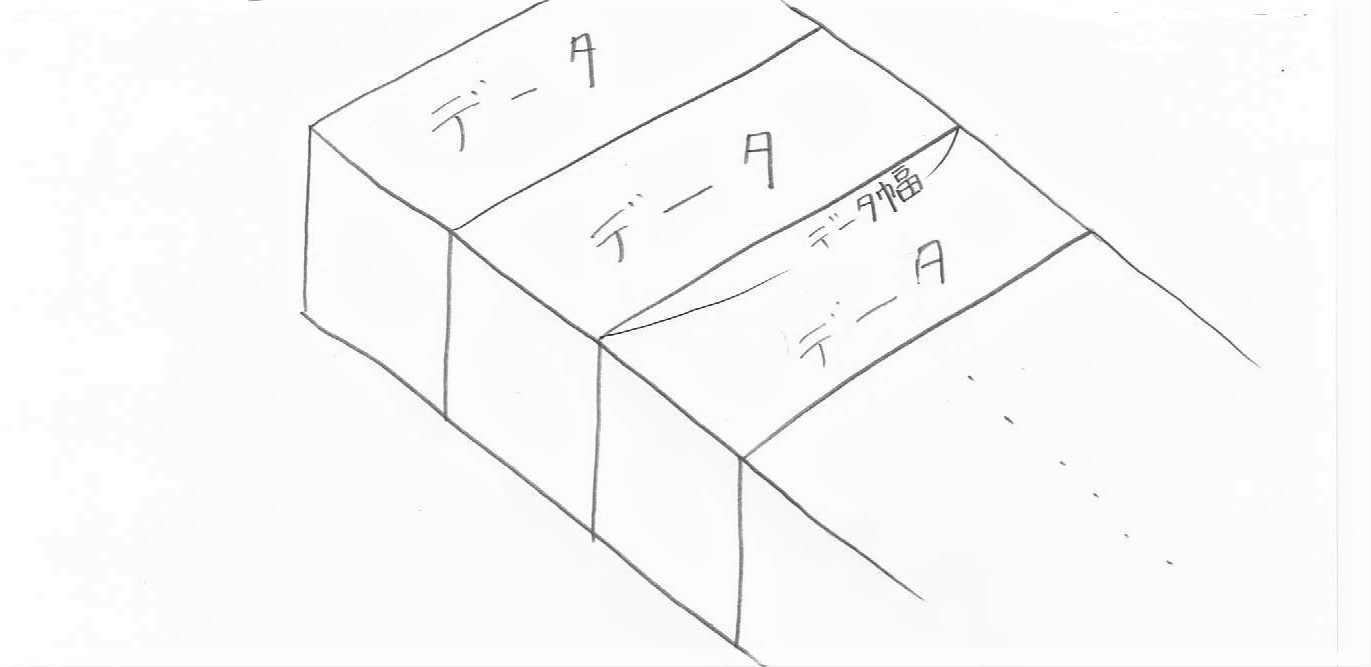
\includegraphics[height=4.5cm]{honda/image/1.jpeg}
\end{figure}
このように棚がズラーっと並んでいるだけなのである。それぞれの棚のなかにはもちろん0,1のデータが入っている。図1のデータ幅というのはこの一つの棚に何個のデータが入るかということで、パソコンなどに使われるメモリは一つの棚にデータが8個入るものが多い。\\
\begin{figure}[H]
  \centering
  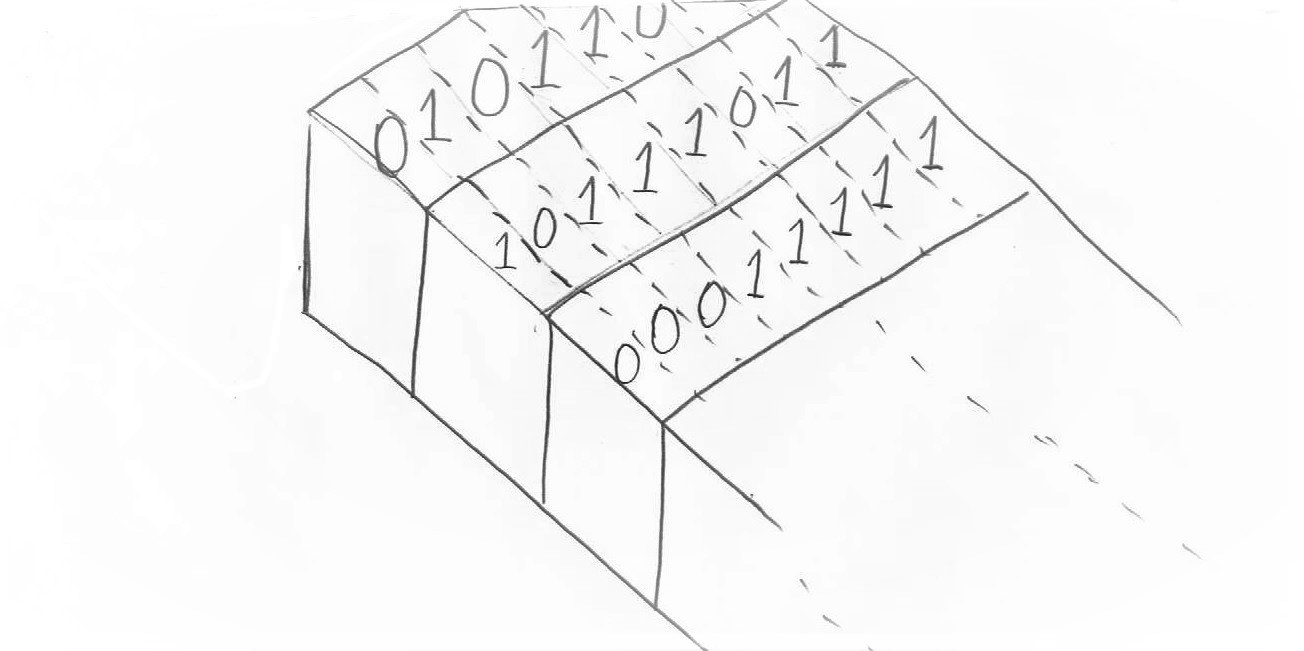
\includegraphics[height=4.5cm]{honda/image/2.jpg}
\end{figure}
この0,1のデータ一つを1bitと呼び、8bitはひとまとめで1Byte(1B)と呼ばれる。\\ 
\begin{figure}[H]
  \centering
  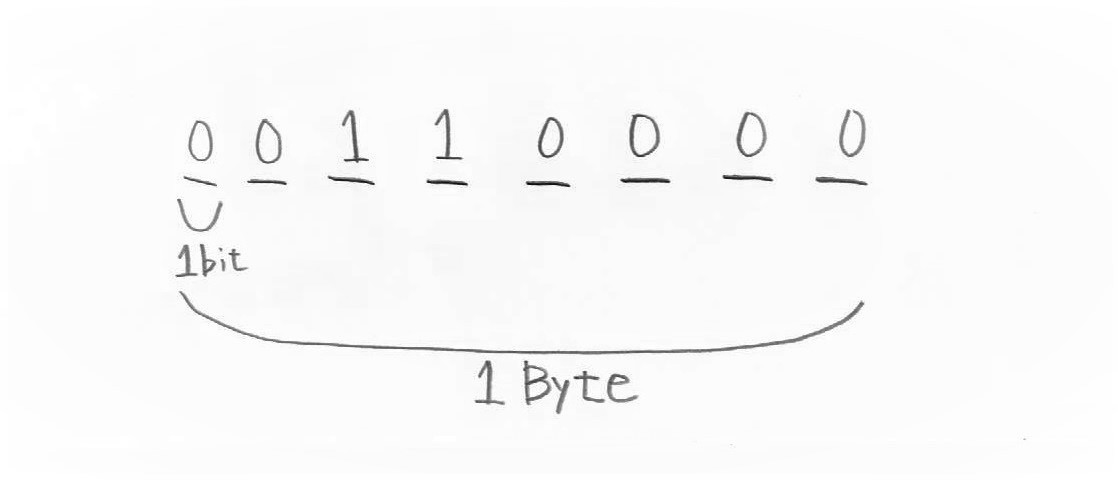
\includegraphics[height=3cm]{honda/image/3.jpeg}
\end{figure}
次にメモリを理解するうえで最も重要な概念、「アドレス」について説明する。アドレスとは英語で「住所」という意味がある。メモリで使うアドレスという言葉も「住所」と同じような使い方をする。先ほど説明した8個のデータが入っている棚一つ一つにそれぞれ番号が振り当てられており、その番号のことをアドレスと呼んでいるのである。
\begin{figure}[H]
  \centering
  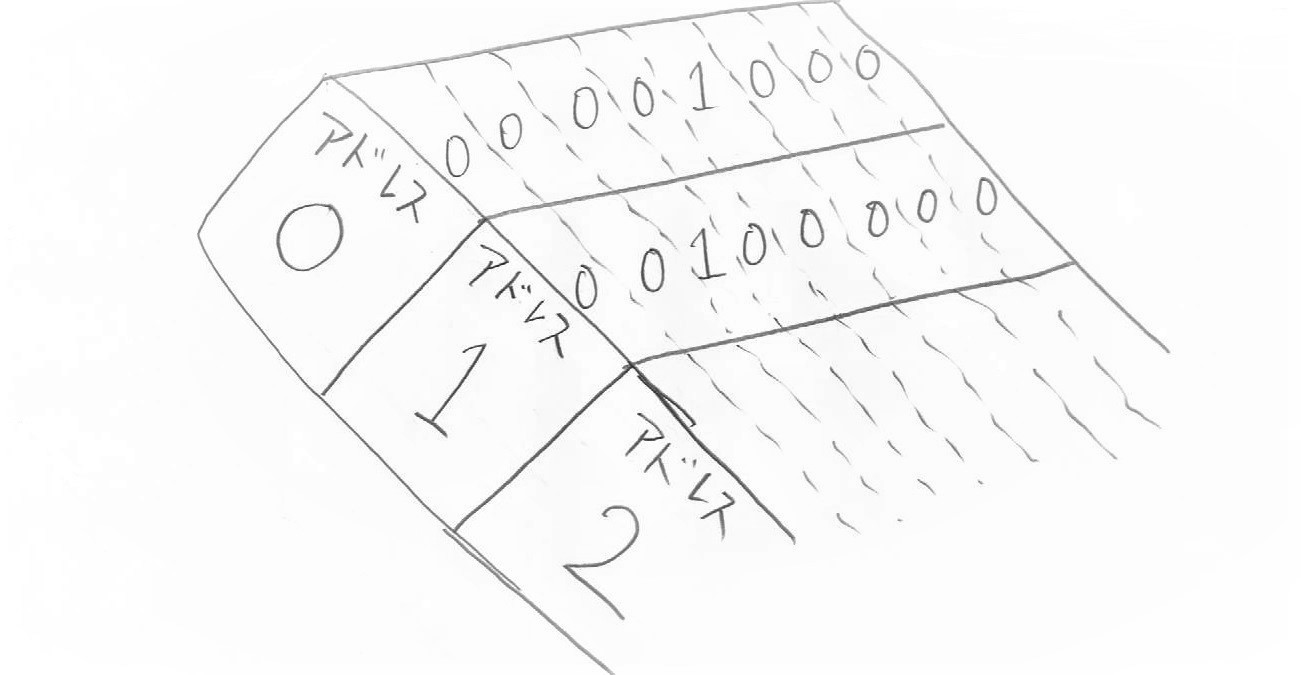
\includegraphics[height=4.5cm]{honda/image/4.jpg}
\end{figure}
上の図ではアドレスを10進数で表したが、実際はコンピュータが扱いやすいように二進数で表現される。また、下図の二進数の0の数はメモリのサイズ(棚の数)によって変わる。
\begin{figure}[H]
  \centering
  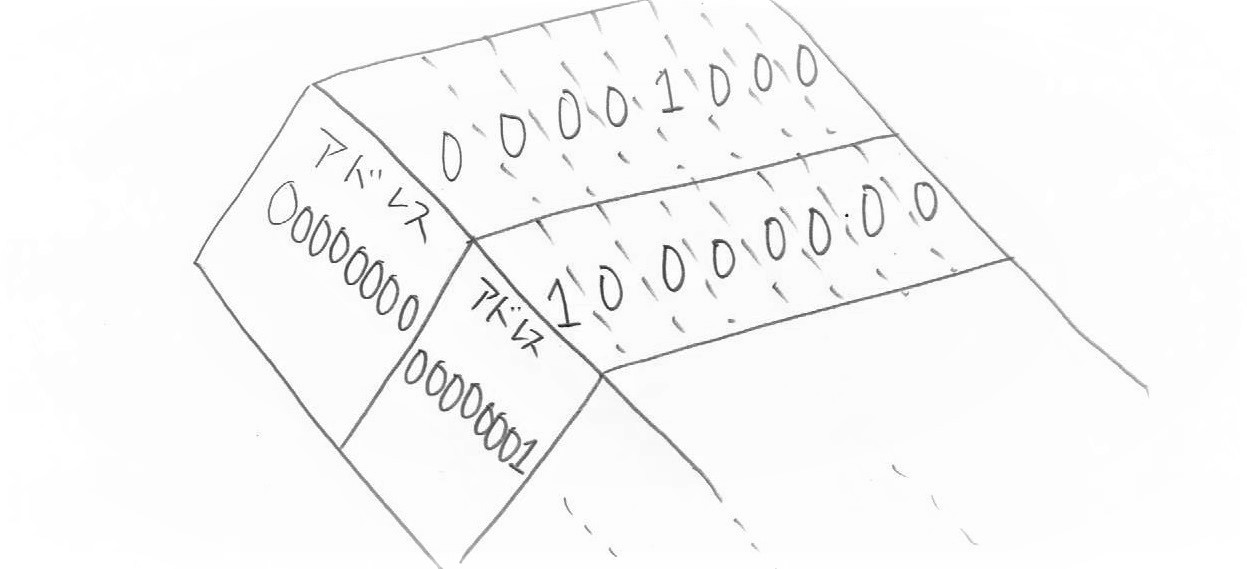
\includegraphics[height=4.5cm]{honda/image/5.jpg}
\end{figure}
大まかなメモリの構造についての説明はこれで終わりで、ここからはより具体的にメモリについて説明する。\\
RAM,ROMについて \\
メモリには大きく分けてRAM,ROMの二種類がある。どちらも構造は先ほど説明した棚のようなものにアドレスが振られているのだが、ROMとRAMでは何が違うのか。\\
ROM…Read Only Memory\\
RAM…Random Access Memory\\
ROM,RAMの略称はこのようになるのだが、これだけ見てもどちらがどのような機能なのかはわからない。ROMとRAMの違いを簡単に説明するなら、「電源を切ったときにデータが消えてしまうか、残ったままか」ということころである。ROMもRAMも電気で動く部品なので、当然動かすには電源が必要である。電源を入れることによってはじめてメモリの中を見たり、書き換えたりできるのである。そして、重要なのはこの電源を「切ったとき」である。ROMの場合それまで入っていたデータが電源を切っても残り続け、次に電源を入れたときは前回のデータのままになっている。\\
\begin{figure}[H]
  \centering
  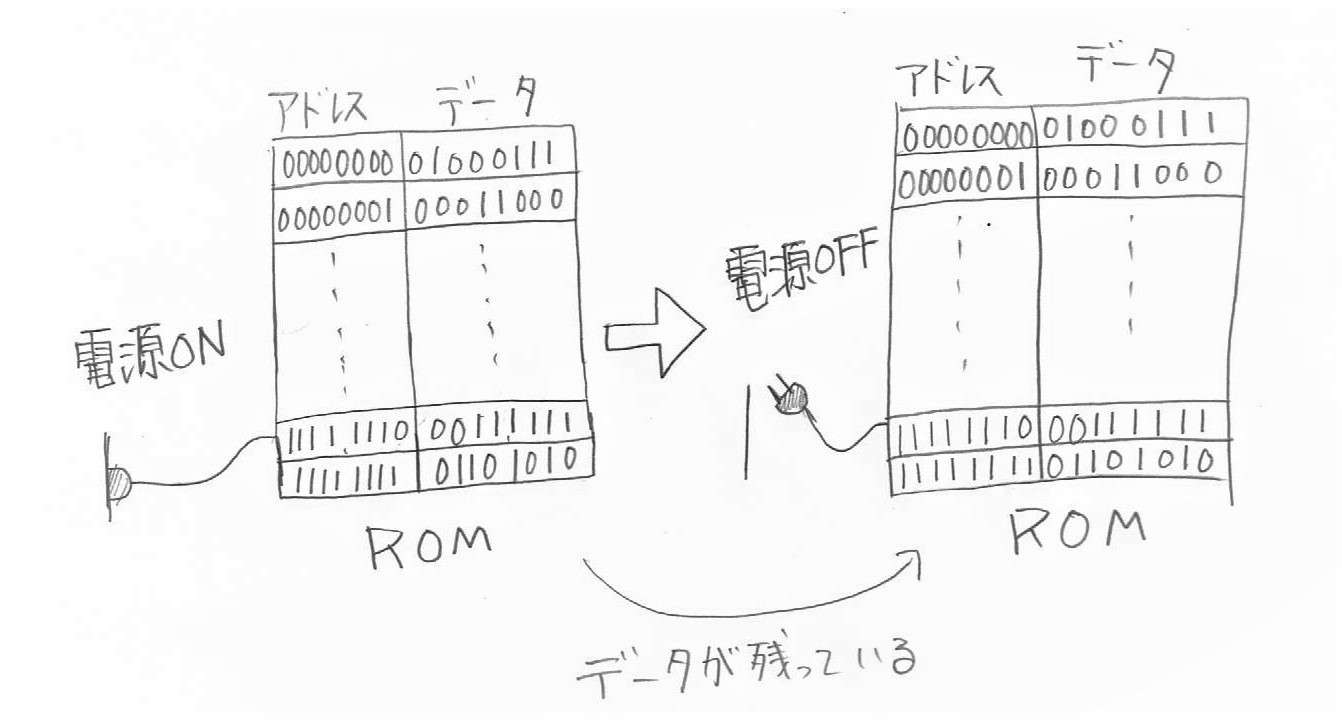
\includegraphics[height=7cm]{honda/image/6.jpeg}
\end{figure}
RAMの場合は1度電源を切ると、それまで入っていたデータは消えてなくなってしまう。では、もう一度電源を入れたときにメモリの中身はどうなっているのか?一度電源を切ってもう一度入れなおしたとき、RAMの中身は全くでたらめな値が入っている。
\begin{figure}[H]
  \centering
  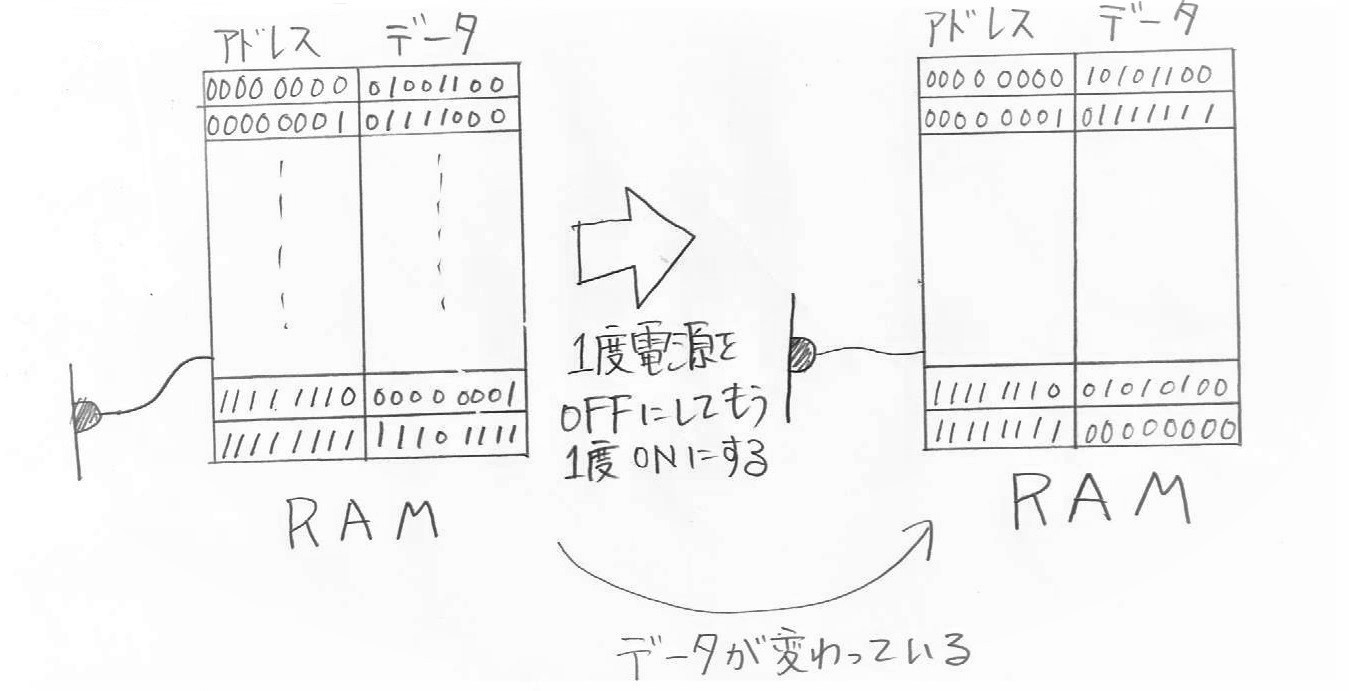
\includegraphics[height=7cm]{honda/image/7.jpg}
\end{figure}
これだけ聞くとRAMよりもROMのほうが役に立ちそうな気もするが、RAM,ROMそれぞれにメリット、デメリットがあり、適材適所に使用される。例を上げればROMはUSBメモリやHDDなどに使われ、RAMはパソコンのスペックを言い表すときに使われる「メモリ」という部分に使われている。\\

\section{レジスタ}
次に、レジスタについて説明する。レジスタというと今まで一度も聞いたことがないという人もいるだろう。簡単に説明するとレジスタもメモリの一種であり、RAMである。では、なぜレジスタという名前を付けて読んでいるのか、それは、CPUの内部にもともと入っている特殊なRAMだからである。ここで初めてCPUの内部の話が出てきたが、CPUの構造について概要を理解してもらうために簡単な概略図を次に示す。\\
\begin{figure}[H]
  \centering
  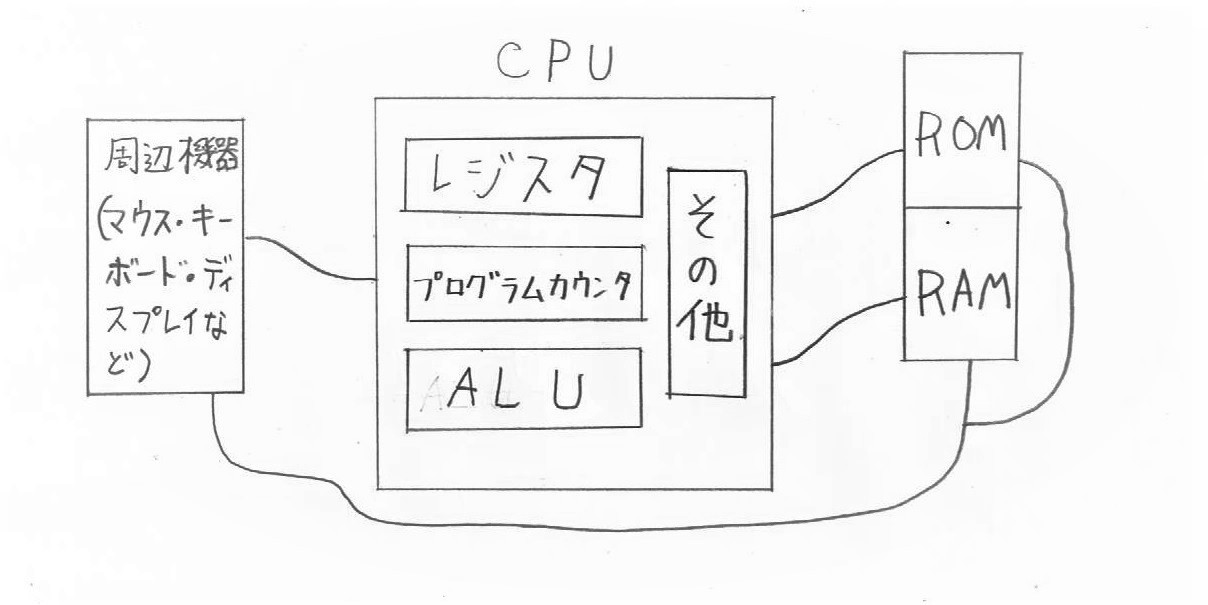
\includegraphics[height=5cm]{honda/image/8.jpeg}
\end{figure}
レジスタは機能的にはほとんどRAMだと思っていい。レジスタの使用例も交えて次の章から改めて解説していく。

\section{機械語}
CPUを動かすためにはCPUにこちらから命令を送らなければならない。CPUは0か1しか取り扱えないので、送る命令は00010110111とか00011111111みたいな命令になってしまう。これを機械語命令というのだが、こんなの人間に理解できるはずがないと思うかもしれない。しかし、そんなこともない。というのも、最新のcore i7~みたいな高機能なCPUならさすがに途方もない量の資料を読み込まないと理解できないとは思うが、まだ動作が単純な頃の古いCPUの機械語なんかだと、それほど苦労することなく理解できたりする。そして、その古いCPUよりもさらに単純な構造で、CPUについてあまり知らない人にもわかりやすいように作られた「自作CPU」というものがある。自作CPUについて書いている本は書店で購入することができ、初心者にとっては非常にとっつきやすいものになっている。今回は、その自作CPUレベルで使用される機械語を使っていくつかのCPUの処理を解説する。
\begin{align*}
0000,0101,0001,0000
\end{align*}
唐突だが、この命令は「内部レジスタに0001,0000を書きこむ」という命令である。もう少し詳しく説明すると、この命令は次のようなブロックに分けて説明することができる。
\begin{figure}[H]
  \centering
  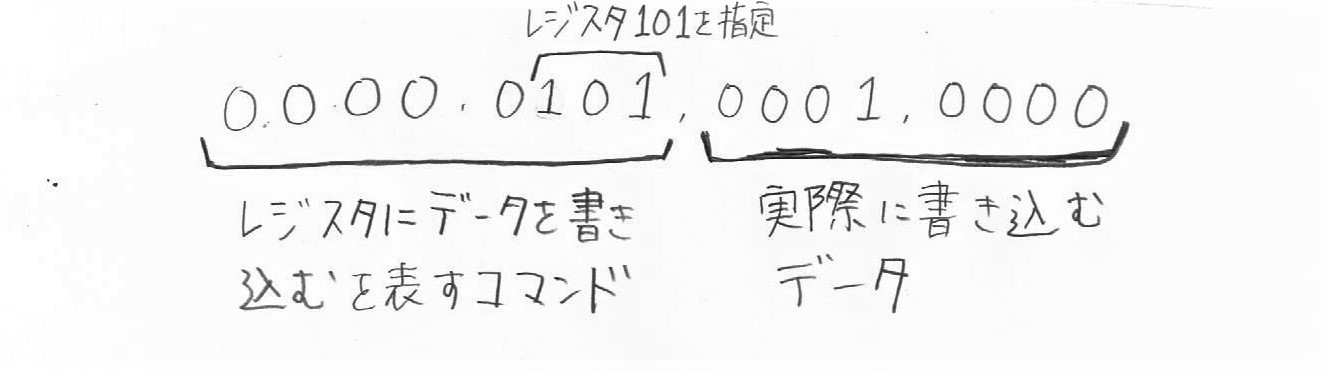
\includegraphics[height=2cm]{honda/image/9.jpg}
\end{figure}
ここで一つ注意してほしいのは、0000,0101が「レジスタにデータを書き込む」という命令を表すといっているが、なにも0000,0101である必要は全くない。今回はわかりやすくするためにこのようにしているが、実際はCPUの回路設計者が決めることである。回路設計者によって0000,0000が「レジスタにデータを書き込む」を意味することもあるし、0000だけで「レジスタにデータを書き込む」を表す場合だってある。その場合、0101が入っていた部分はどうするのかと思うかもしれないが、それも回路設計者によるもので、そこになにが入っても関係ないようなCPUもあれば、そこを細かい追加設定用に使用するCPUもある。しかし、これはあくまで自作CPUレベルの機械語の話であって、実際に使われているCPUはこんなに簡単な話では済まない。\\
ここで、少し話を変えて、レジスタについて説明する。先ほどレジスタについてほとんどRAMと同じだが、少し違うところもあるといったが、その違いは「メモリの数」である。メモリは棚のようなものがずらーっと並んでおり、その一つ一つにアドレスが振られていると言ったが、自作CPUの規模になるとレジスタは数個しかない。つまり、1Byteのデータが入る棚が数個しか並んでないのである。\\
\begin{figure}[H]
  \centering
  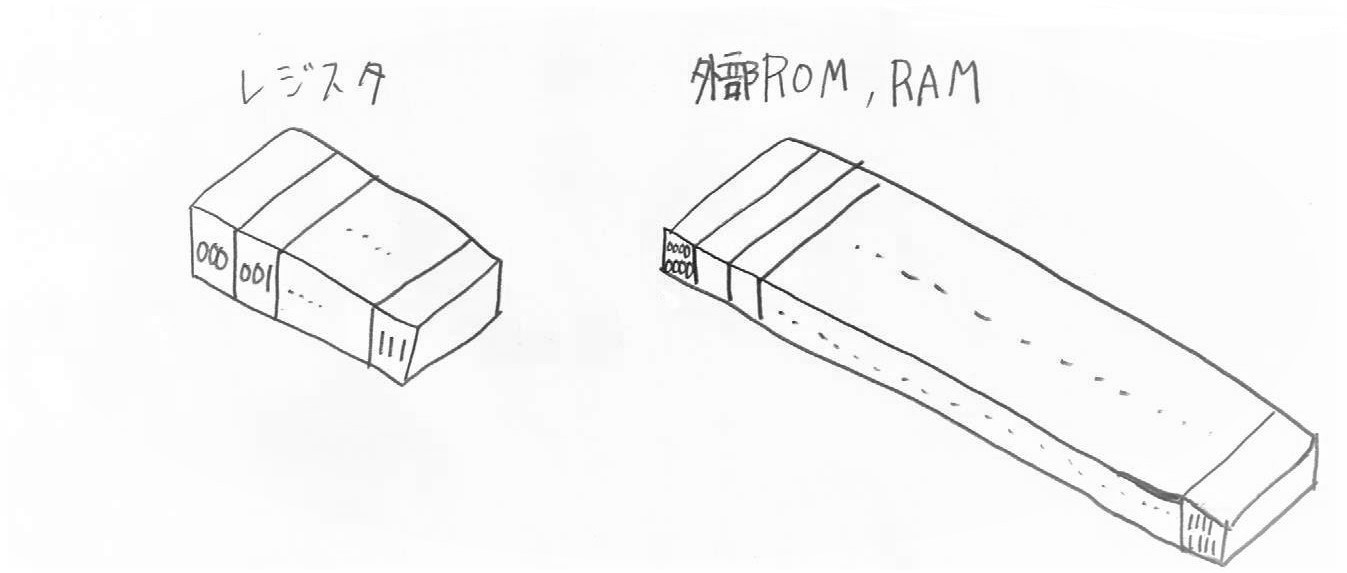
\includegraphics[height=3cm]{honda/image/10.jpg}
\end{figure}
なので、先ほどの機械語ではレジスタ選択に3bitのデータを使っていたので、000~111までの8個のレジスタがあるということになる(実際にレジスタが何個入っているかはCPUによって違う)\\
 先ほどの例と同様にほかの機械語も説明していく。ただし、回路設計上で決める命令の割り当て方についてはあらかじめこちらで決めたものを使うことにし、今回はこのような命令があるということの紹介だけを行うものとする。
\begin{enumerate}
  \item メモリのn番地にレジスタの値を書き込む
  \begin{figure}[H]
    \centering
    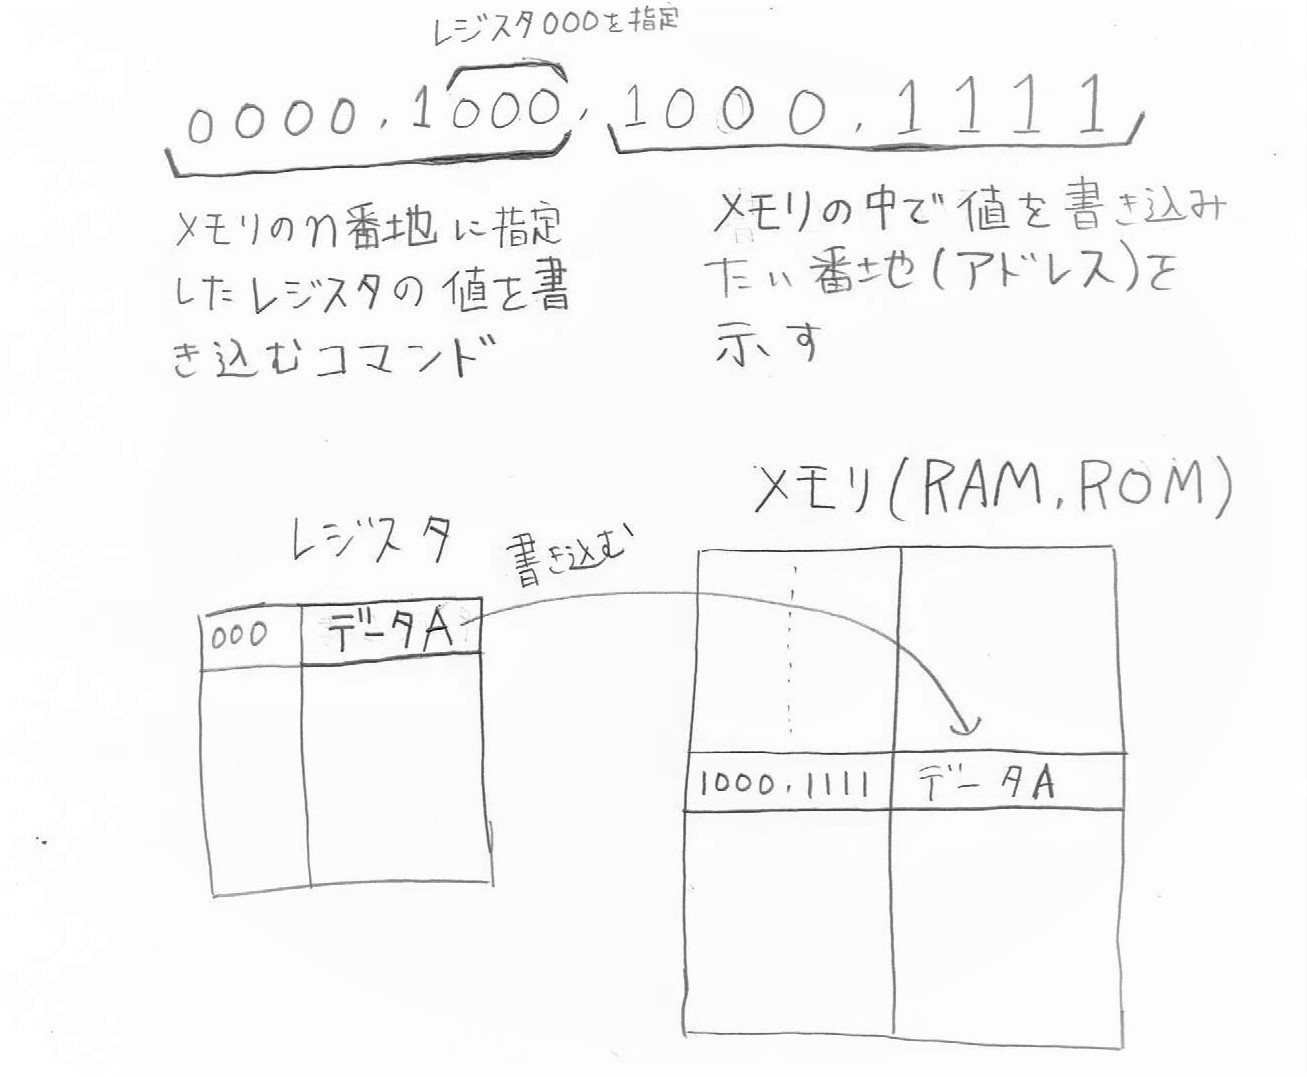
\includegraphics[height=6cm]{honda/image/12.jpg}
  \end{figure}
  この命令を先ほどのレジスタにデータを書き込む命令と一緒に使えば、メモリの好きな場所に好きなデータを書き込むことができる
  \item	メモリのn番地のデータをレジスタに読み出す
  \begin{figure}[H]
    \centering
    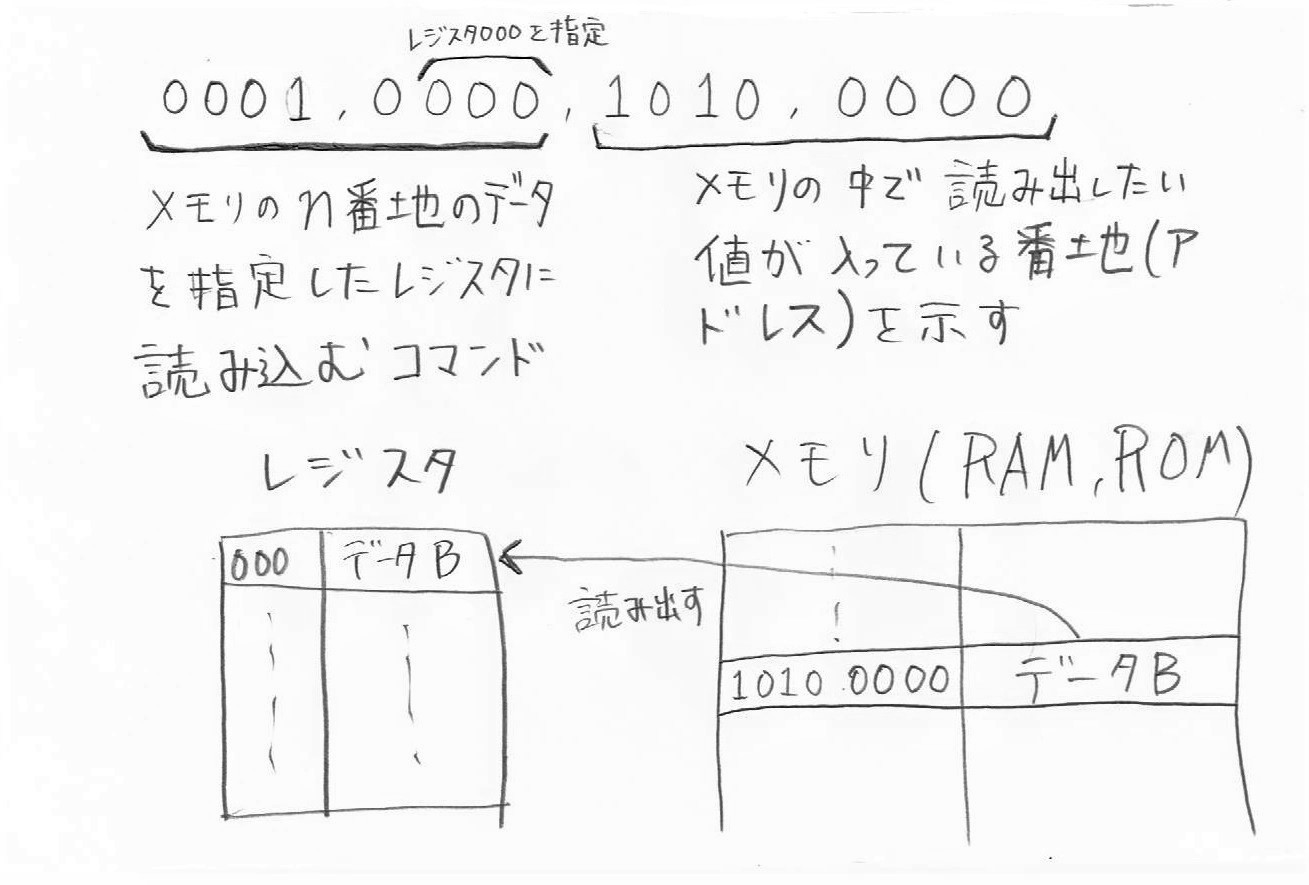
\includegraphics[height=6cm]{honda/image/13.jpg}
  \end{figure}
  この命令でメモリ上のどのデータでも確認することができる
  \item レジスタの値に任意のデータを足し算する
  \begin{figure}[H]
    \centering
    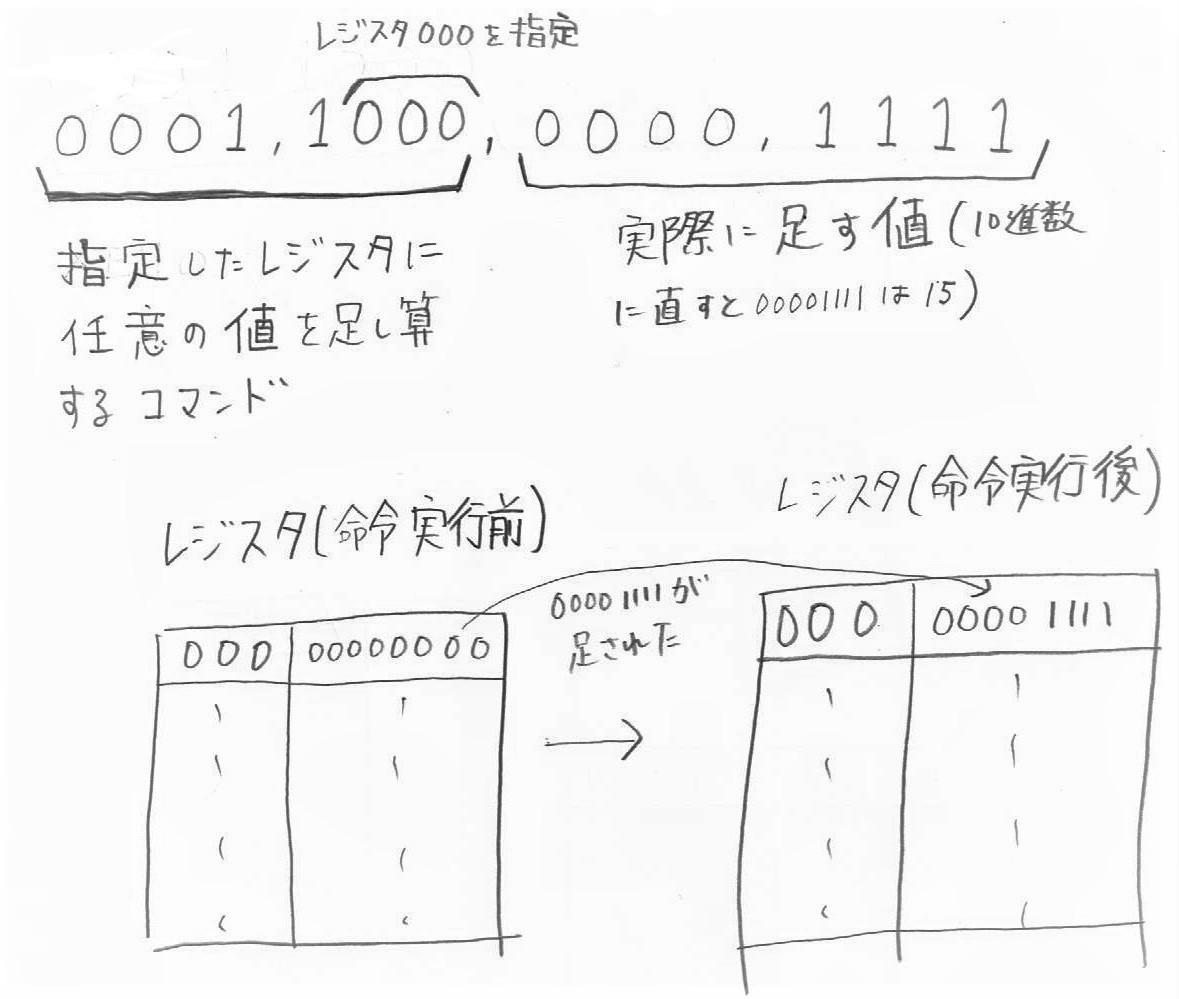
\includegraphics[height=6cm]{honda/image/11.jpg}
  \end{figure}
  引き算も用意されており、掛け算や割り算は足し算、引き算を繰り返すことで実装する。
\end{enumerate}
これだけでは漠然としていてなにができるのかよくわからないかもしれないが、これらの命令を使用するうえで重要なプログラムカウンタという概念について次に説明する。
\section{プログラムカウンタ}
先ほど説明した命令はCPUの命令のうちほんの少しの部分ではあるが、それでもデータの書き込み、読み出し、足し算や引き算などはできる。しかし、これだけだと電卓と機能はほとんど変わらない。では、CPU特有の機能とは何だろうか。それは「何もしなくても命令を順番に実行してくれること」である。先ほどの説明の通り、CPUで扱う命令は0と1のデータである、ということは、メモリの中に保存することができる。なので、CPUを動かすための命令のデータはすべてメモリの中に書き込まれているのである。\\
ここで、「CPUはいったいどこの命令から実行していくのか」と疑問に思ったひとがいると思う。それを決めるのがCPUのプログラムカウンタという部分だ。プログラムカウンタが何をしているかといえば、簡単に説明すると、「メモリの中のどのアドレスの部分の命令を実行するかを指し示すもの」である。ずらーっと並んでいる棚の中から、どれか2つ(今回説明で使った機械語は16bitのデータなので、今回は棚2つ分)が命令として使われる。そのどれかを示しているのがプログラムカウンタなのだが、このプログラムカウンタの賢いところが、命令が一つ実行されるたびに現在の値から1命令分(今回だと棚2つ分)値が増えるのだ。こうすることによってずっと同じ命令を繰り返すのではなく、次から次へと命令を順番に実行していくことができる。またプログラムカウンタは電源を入れた直後は0を示しており、メモリの一番初めに入っている命令を実行することになる。電卓の場合、0を入力、1を足すなどの命令を実行するのにわざわざ指でボタンを押さないといけない。しかし、CPUの場合、メモリの上からレジスタに0を書き込む、1を足すなどの命令を入れておけばいちいちボタンを押さなくても勝手に順番に実行していってくれるし、1秒間に100や1000もの命令を実行することができるので、大量の命令を瞬時にこなすことができ、電卓とは比べ物にならない性能を持っていることがわかる。\\
\begin{figure}[H]
  \centering
  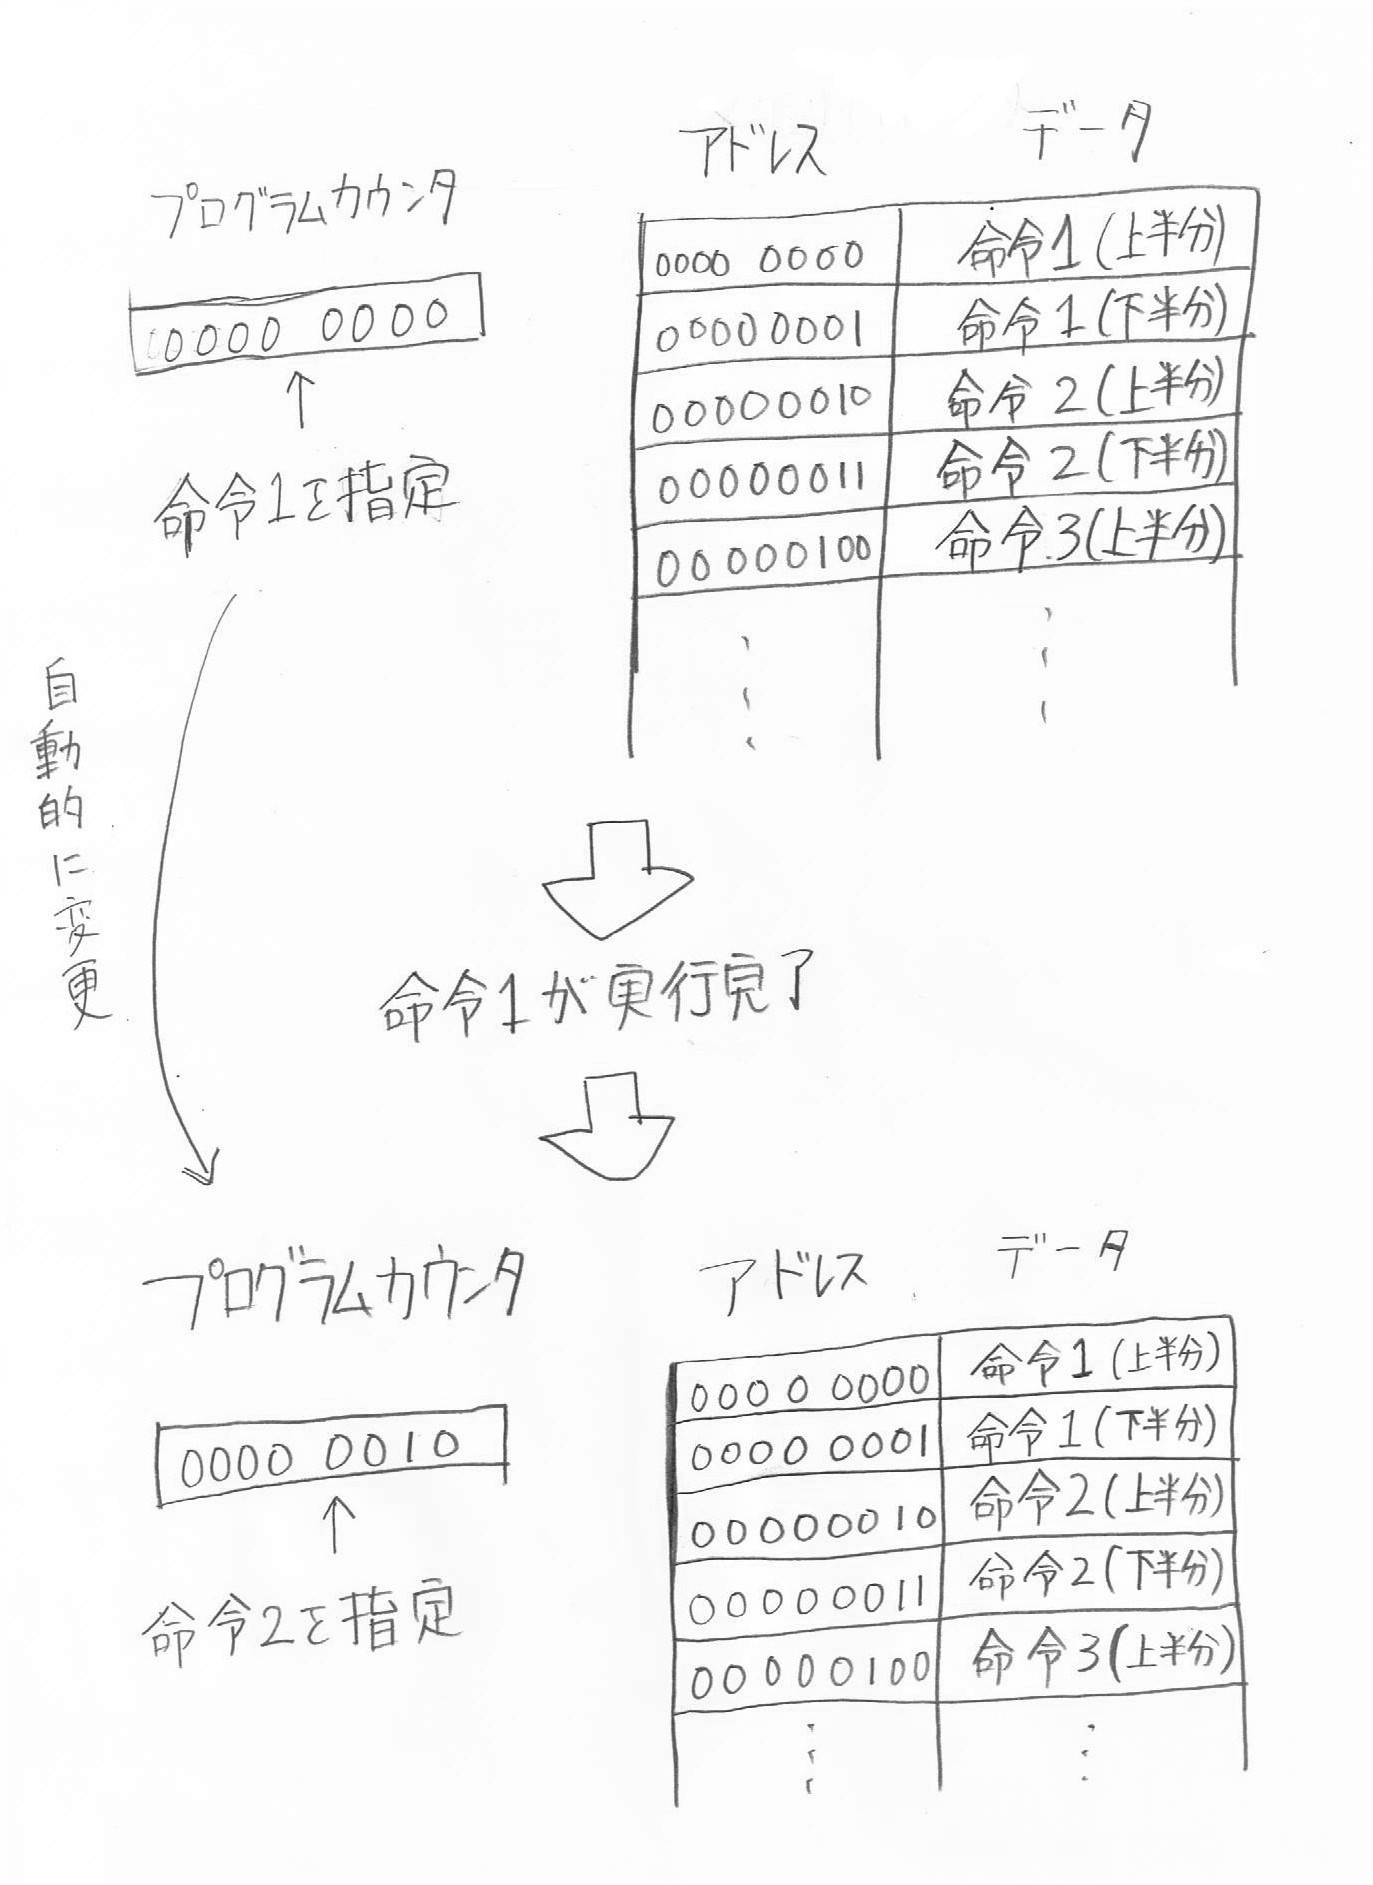
\includegraphics[height=7cm]{honda/image/14.jpg}
\end{figure}
\section{まとめ}
ここまでCPUについていろいろ解説してきたが、これだけではCPUを使えばosを動かしたり、ゲームをしたり、動画を見れたりすることの説明には全くならない。そのようなことはもっといろいろな知識がないと理解できない。しかし、今回私が伝えたかったのはCPUの動作の中でも一番基本の「CPUとメモリの関係」の部分であり、これを理解しているのとしていないのではCPUに対する理解度はかなり違うと思う。これまでCPUが何をしているのかなどまったく気にしたことがなかった人にも、少しCPUについて分かった気になってもらえたらうれしい。\\


%参考文献
%thebibliographyは使わないでください。\chapterになっちゃう!
\section*{参考文献}
\begin{enumerate}
  \item 渡波郁著,CPUの作り方
\end{enumerate}
